\noindent
\section{Prediction results}
\label{result}
In this section, we provide detailed results of the our prediction framework on the datasets discussed earlier.
To determine the accuracy of our prediction strategy we use the cross validation technique.  
For each time step in this range we 
use our framework to obtain a prediction at that time step. Since we already know the original value, we can obtain a percentage error for the prediction.
Let $predict_{t}$ represent the prediction value at time $t$ and $original_{t}$ represent the original value. We obtain percentage error ($error_{t}$) using the formula:
\begin{center}
 {\large$error_{t}=\frac{|original_{t}-predict_{t}|}{original_{t}}*100$}
\end{center}

First we try to find the suitable window for predicting the value of a time series at a time step. For this we refer to figure ~\ref{aging} where 
we quantify structural correlation and show how the similarity value decreases with increasing lag.
We observe that the value of the structural correlation decreases as we increase the lag. For INFOCOM 2006 dataset (figure ~\ref{aging}(A)) the correlation drops to less than 
$0.2$ at lag around $70$.
Therefore we select a window of size 64. 
We could have selected any other value between 60 and 70, but we select 64 as it is in the power of 2 and it helps in the spectrogram 
analysis. Similarly we find the suitable window size to be around 128, 64, 64, 32 (closest power of 2) 
for the SIGCOMM 2009, Highschool 2011, Highschool 2012 and Hospital datasets respectively (refer to figure ~\ref{aging}). 
% If we look into the behavior in figure ~\ref{aging}(B)
%  we observe that even at lag 1 the similarity value is 0.025 and it decreases as we increase lag. We found similar behavior for Facebook posts dataset
%  as well. This essentially suggests that structural correlation does not exist in case networks representing human contact through social media. 
%  Hence we do not find a suitable window for applying our prediction framework in these networks. 
%\subsubsection{Human face-to-face interaction}

%We apply our prediction framework on (i) INFOCOM 2006 and (ii) SIGCOMM 2009 datasets.
For the INFOCOM 2006 dataset we consider the time steps 200-800. 
%We select the range from 200-800 to remove inconsistencies in the series during the initial and also towards the final stages. 
Note that selection of these is just representative and one is free to take 
any time step given there is a window of appropriate length available. For SIGCOMM 2009, High School 2012, High School 2011 and Hospital datasets we 
consider our test time steps to be 300-900, 200-1000, 200-1000 and 100-900 respectively (refer to table 1). 
% for Twitter hashtag co-occurrence dataset we consider the time steps 100-600.
%  We do not apply our prediction framework for the Facebook posts data.
% For each time step in this range we 
% use our framework to obtain a prediction at that time step. Since we already know the original value, we can obtain a percentage error for the prediction.
% Let $predict_{t}$ represent the prediction value at time $t$ and $original_{t}$ represent the original value. We obtain percentage error ($error_{t}$) using the formula:
% \begin{center}
%  {\large$error_{t}=\frac{|original_{t}-predict_{t}|}{original_{t}}*100$}
% \end{center}

\begin{table*}
%\begin{center}
\centering
\begin{adjustbox}{max width=\textwidth}
\begin{tabular}{|c|c|c|c|c|c|}
\hline
                                                                  & \multicolumn{5}{c|}{Prediction error $\leq 20\%$}                                                                                                                                                                                                        \\ \hline
Datasets                                                          & \begin{tabular}[l]{@{}l@{}}INFOCOM \\ 2006\end{tabular} & \begin{tabular}[l]{@{}l@{}}SIGCOMM \\ 2009\end{tabular} & \begin{tabular}[c]{@{}l@{}}Highschool\\ 2012\end{tabular} & \begin{tabular}[c]{@{}l@{}}Highschool\\ 2011\end{tabular} & Hospital \\ \hline
\# Active nodes                                                   & {\bf 0.984}, (0.988)                                                  & {\bf 0.907}, (0.91)                                                   & 0.68, (0.765)                                                      & {\bf 0.861}, (0.882)                                                     & 0.782, (\underline{\it 0.859})    \\ \hline
Average degree                                                    & {\bf 0.975}, (0.968)                                                  & {\bf 0.84}, (0.834)                                                    & {\bf 0.816}, (0.81)                                                     & {\bf 0.91}, (0.908)                                                      & 0.714, (0.724)    \\ \hline
Modularity                                                        & {\bf 0.905}, (0.921)                                                  & {\bf 0.838}, (0.85)                                                   & {\bf 0.90}, (0.91)                                                      & {\bf 0.92}, (0.917)                                                      & 0.78, (0.812)     \\ \hline
Edge emergence                                                    & {\bf 0.971}, (0.983)                                                  & {\bf 0.906}, (0.91)                                                   & 0.56, (\underline{\it 0.71})                                                      & 0.42, (\underline{\it 0.512})                                                      & 0.57, (\underline{\it 0.652})     \\ \hline
\# Active edges                                                   & {\bf 0.901}, (0.91)                                                   & 0.71, (\underline{\it 0.81})                                                    & 0.72, (\underline{\it 0.78})                                                      & {\bf 0.836}, (0.86)                                                     & 0.734, (\underline{\it 0.796})    \\ \hline
\begin{tabular}[c]{@{}l@{}}Clustering \\ coefficient\end{tabular} & {\bf 0.829}, (0.858)                                                  & 0.725, (0.75)                                                   & 0.54, (\underline{\it 0.623})                                                      & 0.5, (\underline{\it 0.682})                                                       & 0.71, (\underline{\it 0.751})     \\ \hline
\begin{tabular}[c]{@{}l@{}}Closeness \\ centrality\end{tabular}   & 0.751, (\underline{\it 0.887})                                                  & 0.71, (\underline{\it 0.83})                                                    & {\bf 0.83}, (0.843)                                                      & {\bf 0.821}, (0.853)                                                     & 0.74, (\underline{\it 0.786})     \\ \hline
\begin{tabular}[c]{@{}l@{}}Betweenness\\ centrality\end{tabular}  & 0.621, (\underline{\it 0.818})                                                  & 0.472, (\underline{\it 0.61})                                                   & 0.51, (0.63)                                                      & 0.22, (\underline{\it 0.418})                                                      & 0.542, (\underline{\it 0.689})    \\ \hline
\hline
Average                                                           & 0.867, (\underline{\it 0.916})                                                  & 0.763, (\underline{\it 0.813})                                                   & 0.694, (\underline{\it 0.768})                                                     & 0.686, (\underline{\it 0.754})                                                     & 0.69, (\underline{\it 0.74})    \\ \hline
\end{tabular}
\end{adjustbox}
 \caption{\label{tab_res}Network property and the fraction of predictions with percentage error  $\leq20\%$ without (with) spectrogram analysis. 
 The cases where more than $80\%$ of the points have prediction error $\leq 20\%$ have been highlighted in bold font and the cases where on using spectrogram analysis 
 the improvement is more than $5\%$ have been underlined.}

\end{table*}
%-eps-converted-to.pdf
\begin{figure}
 \begin{center}
 \includegraphics[width=0.89\columnwidth, angle=0]{./texfiles/Chapter_1/fig/psd_pred-eps-converted-to.pdf}
 \caption{\label{k1}(A) LPSD versus mean percentage error for all the properties across all the datasets.}
  \end{center}
 \end{figure}


 \begin{figure}[!ht]
  \begin{center}
  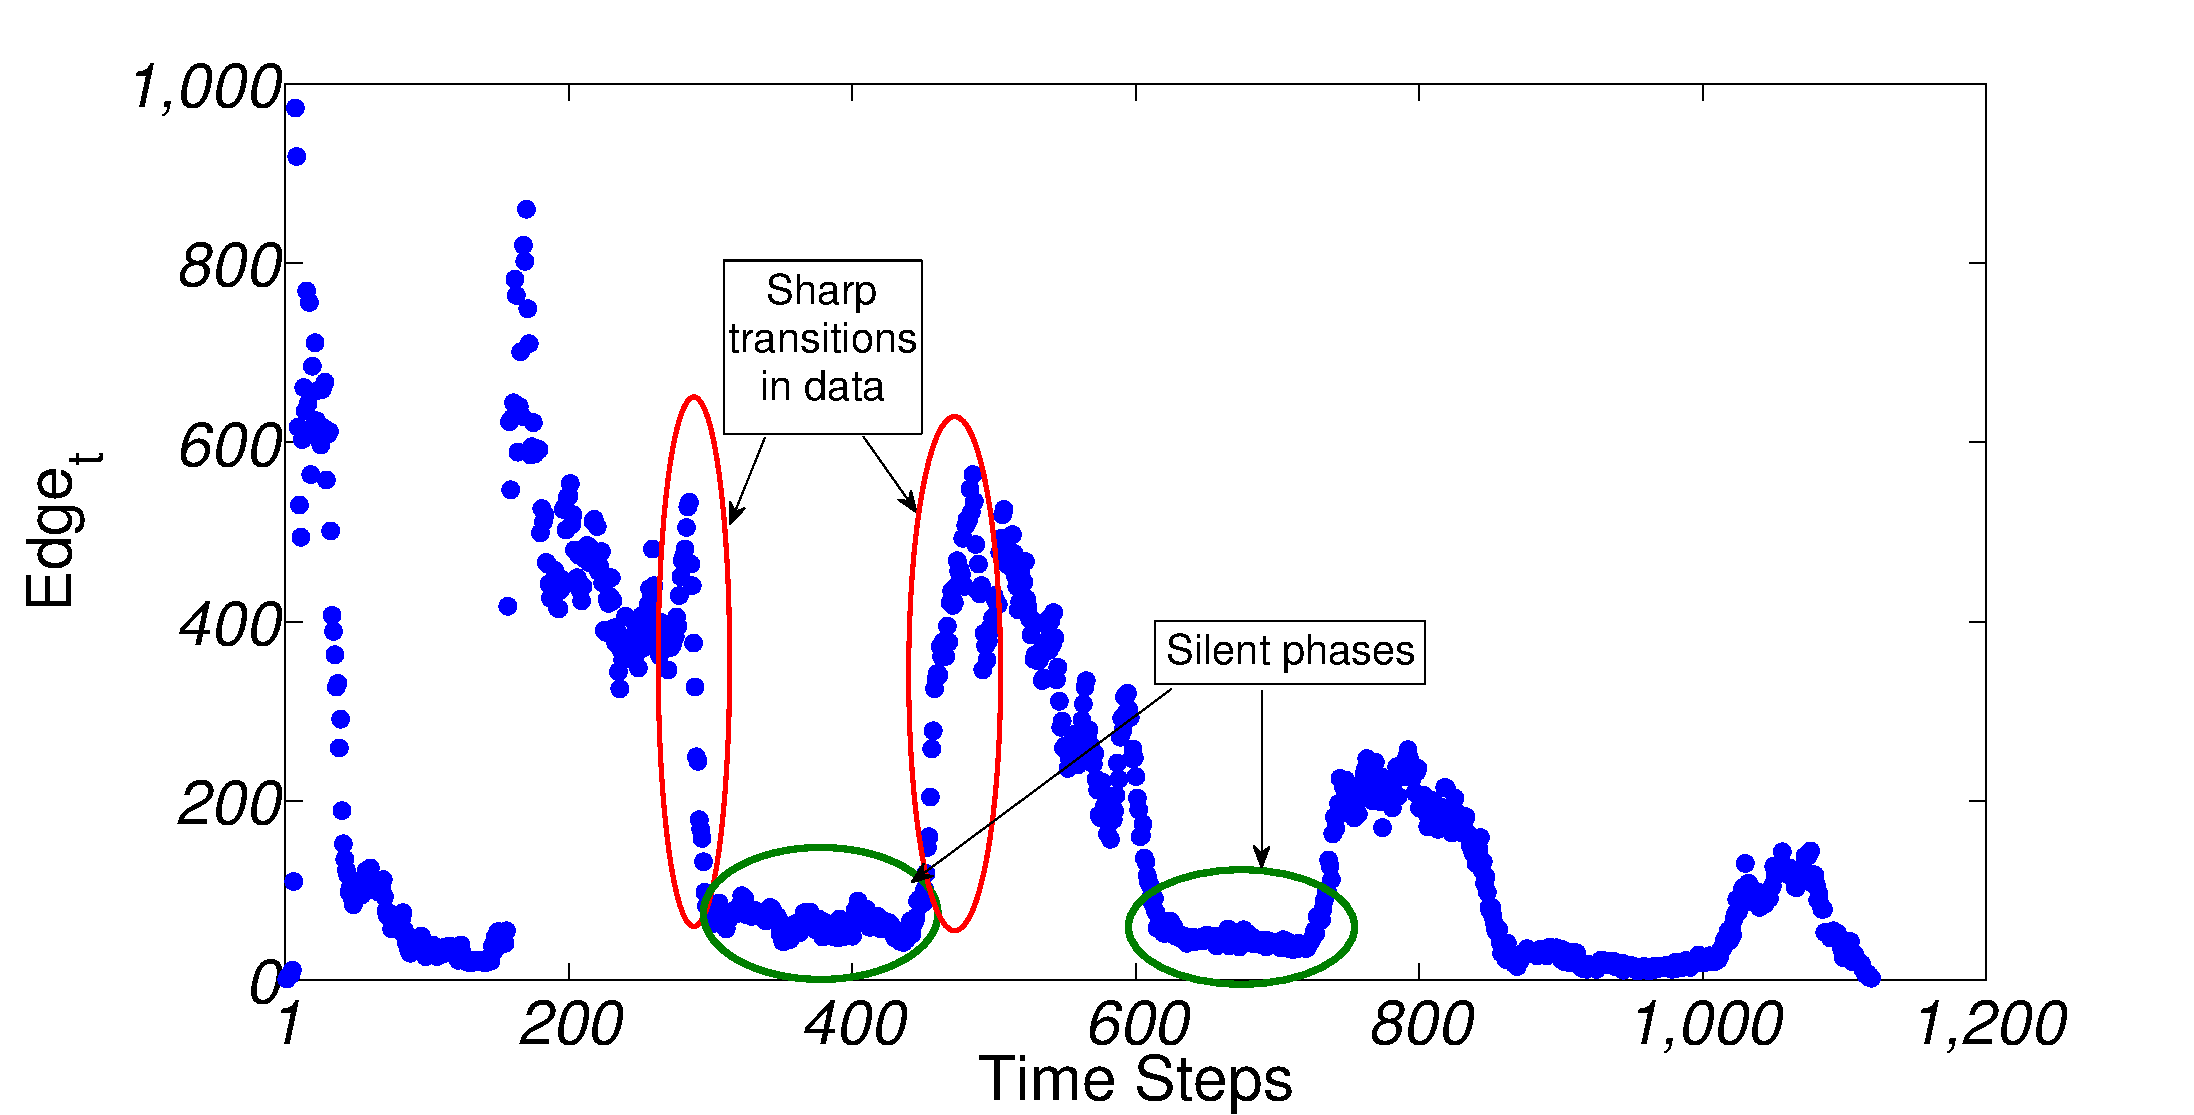
\includegraphics[width=0.7\columnwidth, angle=0]{./texfiles/Chapter_1/fig/no_of_edges1-eps-converted-to.pdf}
  \caption{\label{fig9}The time series plot for number of active edges. The red and the green ellipses identify
  two transition and two silent phases respectively}
  \end{center}
 \end{figure}

%  \begin{figure}
%  \begin{center}
%  \includegraphics[width=0.89\columnwidth, angle=0]{fig/psd_pred-eps-converted-to.pdf}
%  \caption{\label{k1}(A) LPSD versus mean percentage error for all the properties across all the datasets.}
%   \end{center}
%  \end{figure}
%\todo{Make Fig 10 more square -- otherwise difficult to understand}
 
 \begin{figure}[!ht]
  \begin{center}
  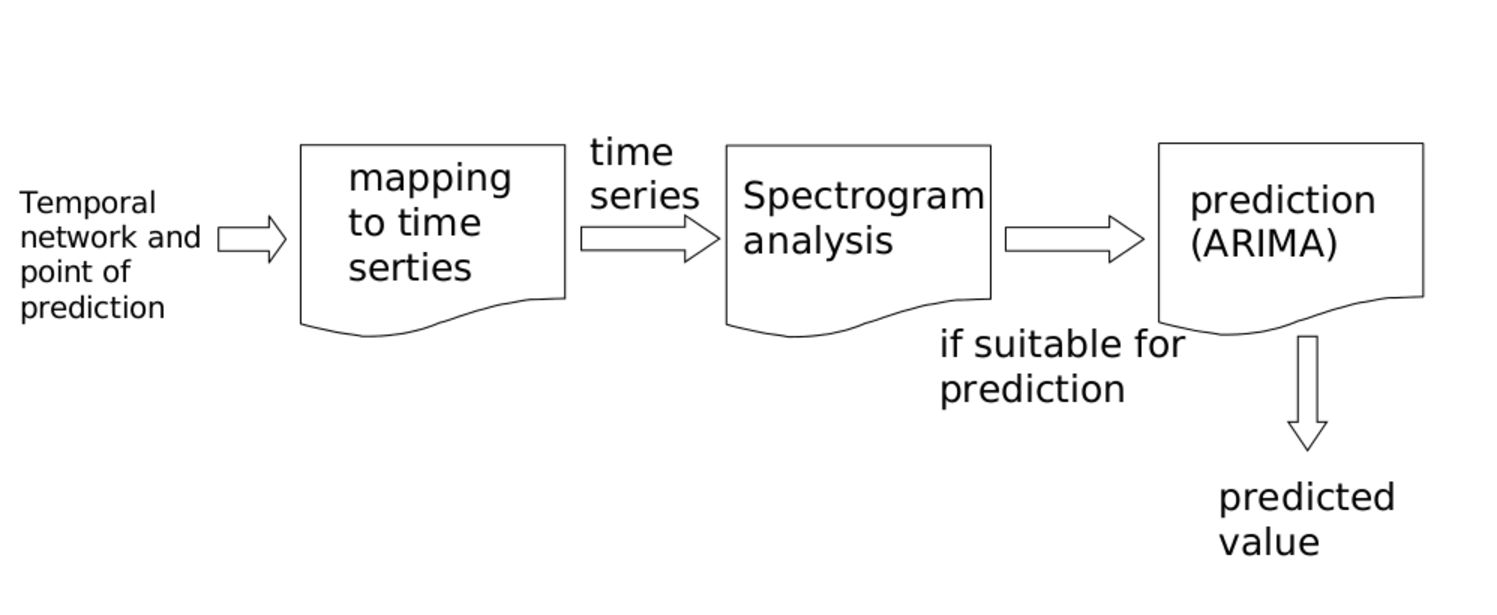
\includegraphics[width=0.95\columnwidth, angle=0]{./texfiles/Chapter_1/fig/Prediction.pdf}
  \caption{\label{fig13}The prediction framework.}
  \end{center}
 \end{figure}
 
%\todo{Is Fig 8 a new figure}
 

%\todo{This para is very poorly written}
To check how efficient our predictions are we plot the cumulative probability distribution of percentage error for all the datasets in figure ~\ref{fig8}. 
In table ~\ref{tab_res}, we compare the prediction results across different datasets and different metrics for cases where the prediction error $\leq20\%$. 
 Note that this error level is representative and ideally a table can be recovered for each such error level from figure ~\ref{fig8}. We make the 
 following observations from the results: 
\begin{itemize}
 \item  Our framework is able to predict the values for active nodes, average degree and modularity with high accuracy across all datasets. 
%  In fact the prediction error is 
%  less than or equal to $20\%$ with probability 0.84, 0.85 and 0.86 respectively for active nodes, average degree and modularity on an average across all datasets.
 \item For active edges, edge emergence, clustering coefficient and closeness centrality our framework is able to predict the values with moderate accuracy although the 
 prediction accuracy for these properties is reasonably high for some datasets (INFOCOM 2006, SIGCOMM 2009).
 \item The prediction accuracy is poor across all datasets for betweenness centrality and in some cases for clustering coefficient and closeness centrality.
\end{itemize}


An important observation is that the spectrogram analysis (introduced in section ~\ref{properties}) is able to distinguish between these properties based on their 
 predictability. On ranking the properties based on the PSD value at bin 1 (refer to figures ~\ref{fig_all_dataset}(B), (D), (F) and ~\ref{fig_all_dataset_1}(B), (D)), we observe 
 that the higher ranked properties are the ones for which the prediction error is low while the lower ranked ones have higher prediction error. 
 Following this observation we further plot the mean percentage error for all the properties across all the datasets versus LPSD in figure ~\ref{k1}. 
 The plot clearly shows that the higher the value of LPSD, lower is the 
mean percentage of error and vice versa.
%This shows that spectrogram of the time series can be used to determine whether a property can be predicted with low percentage error in prediction.

On further investigating into the cases where the prediction error is high, we observed that these points are mostly located either in places where a sharp 
 transition occurred or in silent phases where there was limited interaction among the nodes. Figure~\ref{fig9} identifies some of the transition and silent phases 
 in the time series of number of active edges in INFOCOM 2006 dataset.
Similar phases are also present in the other datasets as well. 
 %An immediate extension to check whether we can leverage spectrogram analysis to identify these points beforehand. 
%  To our aim we extend the spectrogram analysis to the single point case whereby  
%  while predicting a property at a give time step, we find that the spectrogram of the window ($w$) and use the LPSD value as an indicator for prediction accuracy. 
% We 

 

%\subsection{Capturing the high error points}
%We next concentrate on the time points where the prediction error is high. 
% For the 600 time steps we considered, only in case of 8 time points for INFOCOM 2006 dataset and 32 time points in case of SIGCOMM 2009 dataset, did we find 
% more than five of the eight properties to give prediction error percentage more than 20\%. 
% \textcolor{blue}{Once again the error level chosen is representative and similar results are obtained for 10\% and 30\% error levels.} 
% For High school 2012, High school 2011 and Hospital datasets the corresponding 
% numbers are 42, 38 and 52 respectively.
% We observe that these points are mostly located either in places where a sharp transition occurred or in silent phases where there was limited interaction among the nodes.
% % On further 
% % investigation we find them to be either in places where a sharp transition has occurred or in the silent phases where there are have been limited interaction among the nodes.
% Figure~\ref{fig9} identifies some of the transition and silent phases in the time series of number of active edges in INFOCOM 2006 dataset.
% Similar phases are also present in the other datasets as well. 
% Next we check whether we can identify these points beforehand.
% These transition phases or silent phases are the idiosyncrasies of the dataset. 
% Since we are using human communication network, transition phases occur mostly due to the bursty nature of the network.
% We believe that our strategy will give even better result for datasets with higher stationarity. 
\begin{figure*}[!ht]
  \begin{center}
  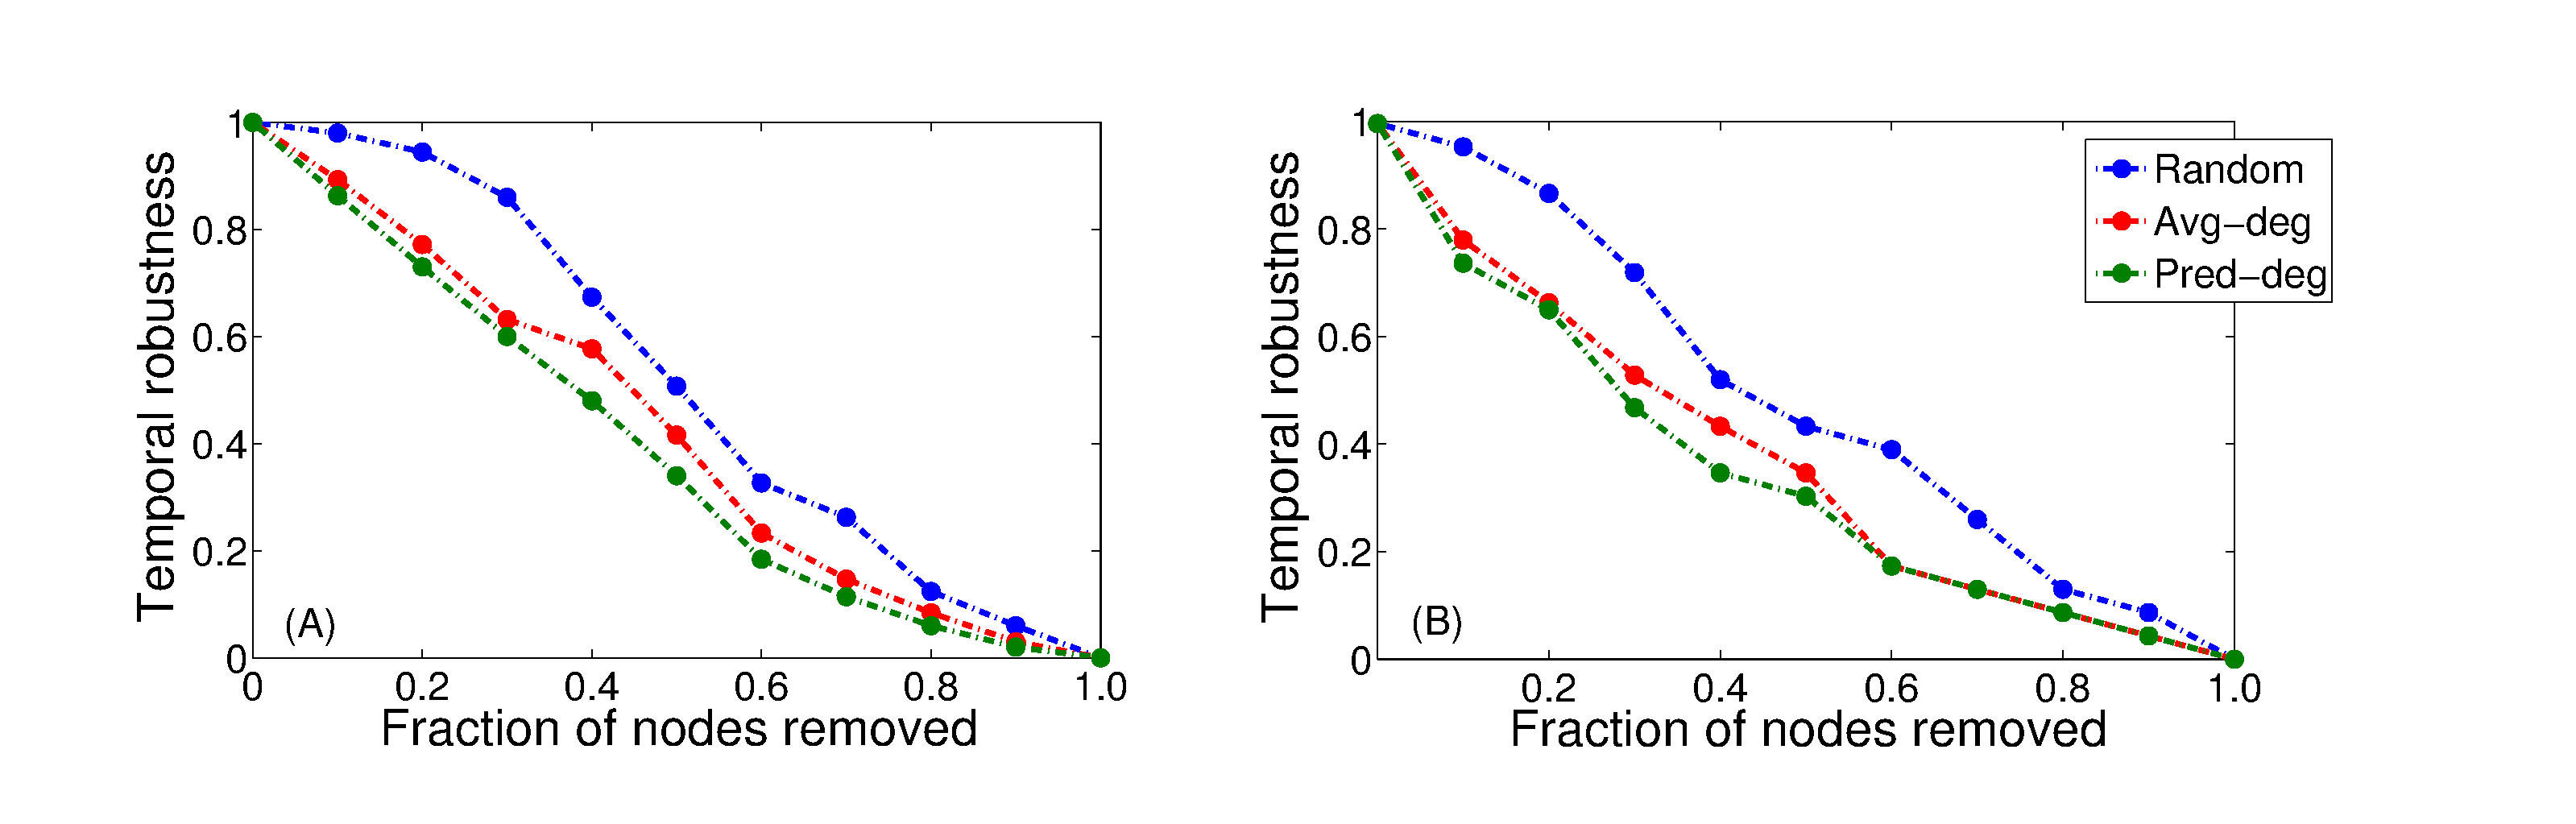
\includegraphics[width=0.9\linewidth, angle=0]{./texfiles/Chapter_1/fig/attack_all-eps-converted-to.pdf}
  \caption{\label{fig_attack}Temporal robustness as a function of the fraction of removed nodes for (a) INFOCOM 2006 and (b) SIGCOMM 2009 datasets.}
  \end{center}
 \end{figure*}

 
% Previously we have seen that spectrogram analysis on the time series of the properties is able to separate out the properties which are predictable (low errors in prediction). 
% We further plot the 
% mean percentage error against the mean PSD of frequencies $<$ 5 Hz (bin 1) in figure ~\ref{k1}(A). The plot clearly shows that the higher the value LPSD lower is the 
% mean percentage error and vice versa. Thus through the spectrogram of the time series we can conclude whether a property can be predicted 
% with low percentage error in prediction.
% To check whether the prediction at a time point would be erroneous, we extend the spectrogram analysis to the single point case. 
% While predicting a property at a give time step, we find that the spectrogram of the window ($w$) can be an 
% indicator for prediction accuracy. To our aim we consider two time steps: one where the prediction error is low and other where it is high for the property 
% number of active edges (INFOCOM 2006 dataset).
% In figure ~\ref{k1}(B) we plot the corresponding mean PSD value for the frequencies $<$ 5 Hz (bin 1) 
% for the two time steps. We observe 
% that the mean PSD value corresponding to the frequencies $<$ 5 Hz (bin 1) to be much higher in case where the prediction error is low (1) than 
% in the case where the prediction error was high (2). In fact this method could identify most of the points which where present in the transition or silent phase. 
% All these observations lead us to believe that spectrogram analysis can be used to filter out cases where the prediction error is high and thereby improve 
% the overall accuracy of our prediction framework.
 
 
 
\subsection{Enhancing the prediction scheme through spectrogram}

Since spectrogram analysis of the time series could determine the predictability of the corresponding property, 
an immediate extension would be to check whether it could be leveraged to identify beforehand the cases where the prediction error is high (unsuitable for prediction). 
To that aim we extend the spectrogram analysis to the single point case whereby  
 while predicting a property at a give time step, we find that the spectrogram of the window ($w$) and use the LPSD value as an indicator for potential prediction accuracy. 
 The cases identified by spectrogram analysis to be unsuitable for prediction can then be filtered out to improve the overall accuracy of the prediction framework. 
  A schematic diagram of this enhanced prediction framework is 
 provided in figure ~\ref{fig13}.
We now consider all the datasets and the corresponding time steps for prediction (which we considered earlier in this section, refer to table 1) and  
instead of directly using our prediction framework we 
 perform spectrogram analysis (single point method) on these points to separate out those which are unsuitable for prediction. We predict 
 only the points which the spectrogram analysis identified as suitable for prediction.
 In table ~\ref{tab_res} we compare the fraction of predictions with 
 error $\leq 20\%$ between both the cases where we do not use spectrogram  and where we use spectrogram. 
 We observe that the fraction of prediction with error $\leq 20\%$ is enhanced for all the properties albeit only marginally in some cases where the accuracy was already high. 
 More importantly for (ill-predicted) properties like betweenness centrality, closeness centrality, the prediction
accuracy increases substantially. 
 Note that prediction error $20\%$ is again representative and similar results 
 could be obtained for other values of prediction error as well.

% \subsubsection{Human interaction through social media}
% 
% \textcolor{blue}{We also applied our framework for the Twitter hashtag co-occurrence (London olympics) dataset for the properties for which short term correlation was present.
% We fixed the range of time steps between 100 and 600 and the average value of the fraction of predictions with percentage error less than or equal to 20\% 
% is 0.48. In table ~\ref{tab_twt} we report the detailed results. 
% As mentioned earlier we donot apply our prediction framework on the Facebook posts dataset.}
% 
% \begin{table}[h]
% \begin{tabular}{|c|c|c|c|c|c|c|}
% \hline
% \multirow{2}{*}{Network features} & \multicolumn{6}{l|}{Percentage error}                                     \\ \cline{2-7} 
%                                   & \multicolumn{3}{l|}{\textless=10\%} & \multicolumn{3}{l|}{\textless=20\%} \\ \hline
% Number of active nodes            & \multicolumn{3}{l|}{0.33}           & \multicolumn{3}{l|}{0.551}           \\ \hline
% Number of active edges            & \multicolumn{3}{l|}{0.294}          & \multicolumn{3}{l|}{0.494}           \\ \hline
% Average degree                    & \multicolumn{3}{l|}{0.276}          & \multicolumn{3}{l|}{0.517}          \\ \hline
% Clustering coefficient            & \multicolumn{3}{l|}{0.216}          & \multicolumn{3}{l|}{0.401}               \\ \hline
% Average            & \multicolumn{3}{l|}{0.275}          & \multicolumn{3}{l|}{0.485}               \\ \hline
% \end{tabular}
% \caption{\label{tab_twt}Network property and the fraction of predictions with percentage error less than or equal to 10\% and 20\% for Twitter hastag co-occurrence 
% network.}
% \end{table}

\medskip
